\documentclass{homework}
\usepackage{siunitx}
\usepackage{graphicx}
\newcommand{\hwname}{Zooey Nguyen}
\newcommand{\hwemail}{zooeyn@ucla.edu}
\newcommand{\hwclass}{Astro 81}
\newcommand{\hwtype}{Homework}
\newcommand{\hwnum}{6}
\begin{document}
\maketitle
\question
Use blackbody approximation to compare temperatures.
\begin{align*}
    1.05	&=  \frac{T_p}{T_a} \\
    1.05    &=	\sqrt{\frac{d_a}{d_p}}	\\
    1.05    &=	\sqrt{\frac{1+e}{1-e}}	\\
    1.1025    &=	\frac{1+e}{1-e}	\\
    1.1025(1-e)    &=	1+e	\\
    0.1025    &=	2.1025e	\\
    e   &=  \boxed{.0487}
\end{align*}


\question
\begin{alphaparts}
    \questionpart Get semi-major axis and then use with orbital period.
    \begin{align*}
        R	&=	\SI{8e3}{pc} \vdot \SI{0.126}{\arcsec}	\\
        R    &=  \SI{1008}{AU}   \\
        M_{BH}    &\propto	\frac{R^3}{P^2}	\\
        M_{BH}    &=	\frac{1008^3}{16^2} M_\odot	\\
        M_{BH}    &=	\boxed{\SI{4e6}{M_\odot}}
    \end{align*}
    About four million Sun masses.
    \questionpart Use equations for apoapse and periapse.
    \begin{align*}
        \frac{r_p}{r_a}	&=	\frac{1-e}{1+e}	\\
        \frac{\ddot{r_p}}{\ddot{r_a}}	&=	\frac{1-e}{1+e}	\\
        20	&=	\frac{1-e}{1+e}	\\
        e   &=  \boxed{0.9047}
    \end{align*}
    \questionpart It might not look consistent at first because such a high eccentricity would usually imply an extremely wide orbit rather than a very short one of just 16 years, but the black hole is so massive that stars like S0-2 will be orbiting extremely quickly.
\end{alphaparts}

\question
\begin{alphaparts}
    \questionpart Binary system diagram.
    \begin{figure}[h]
        \centering
        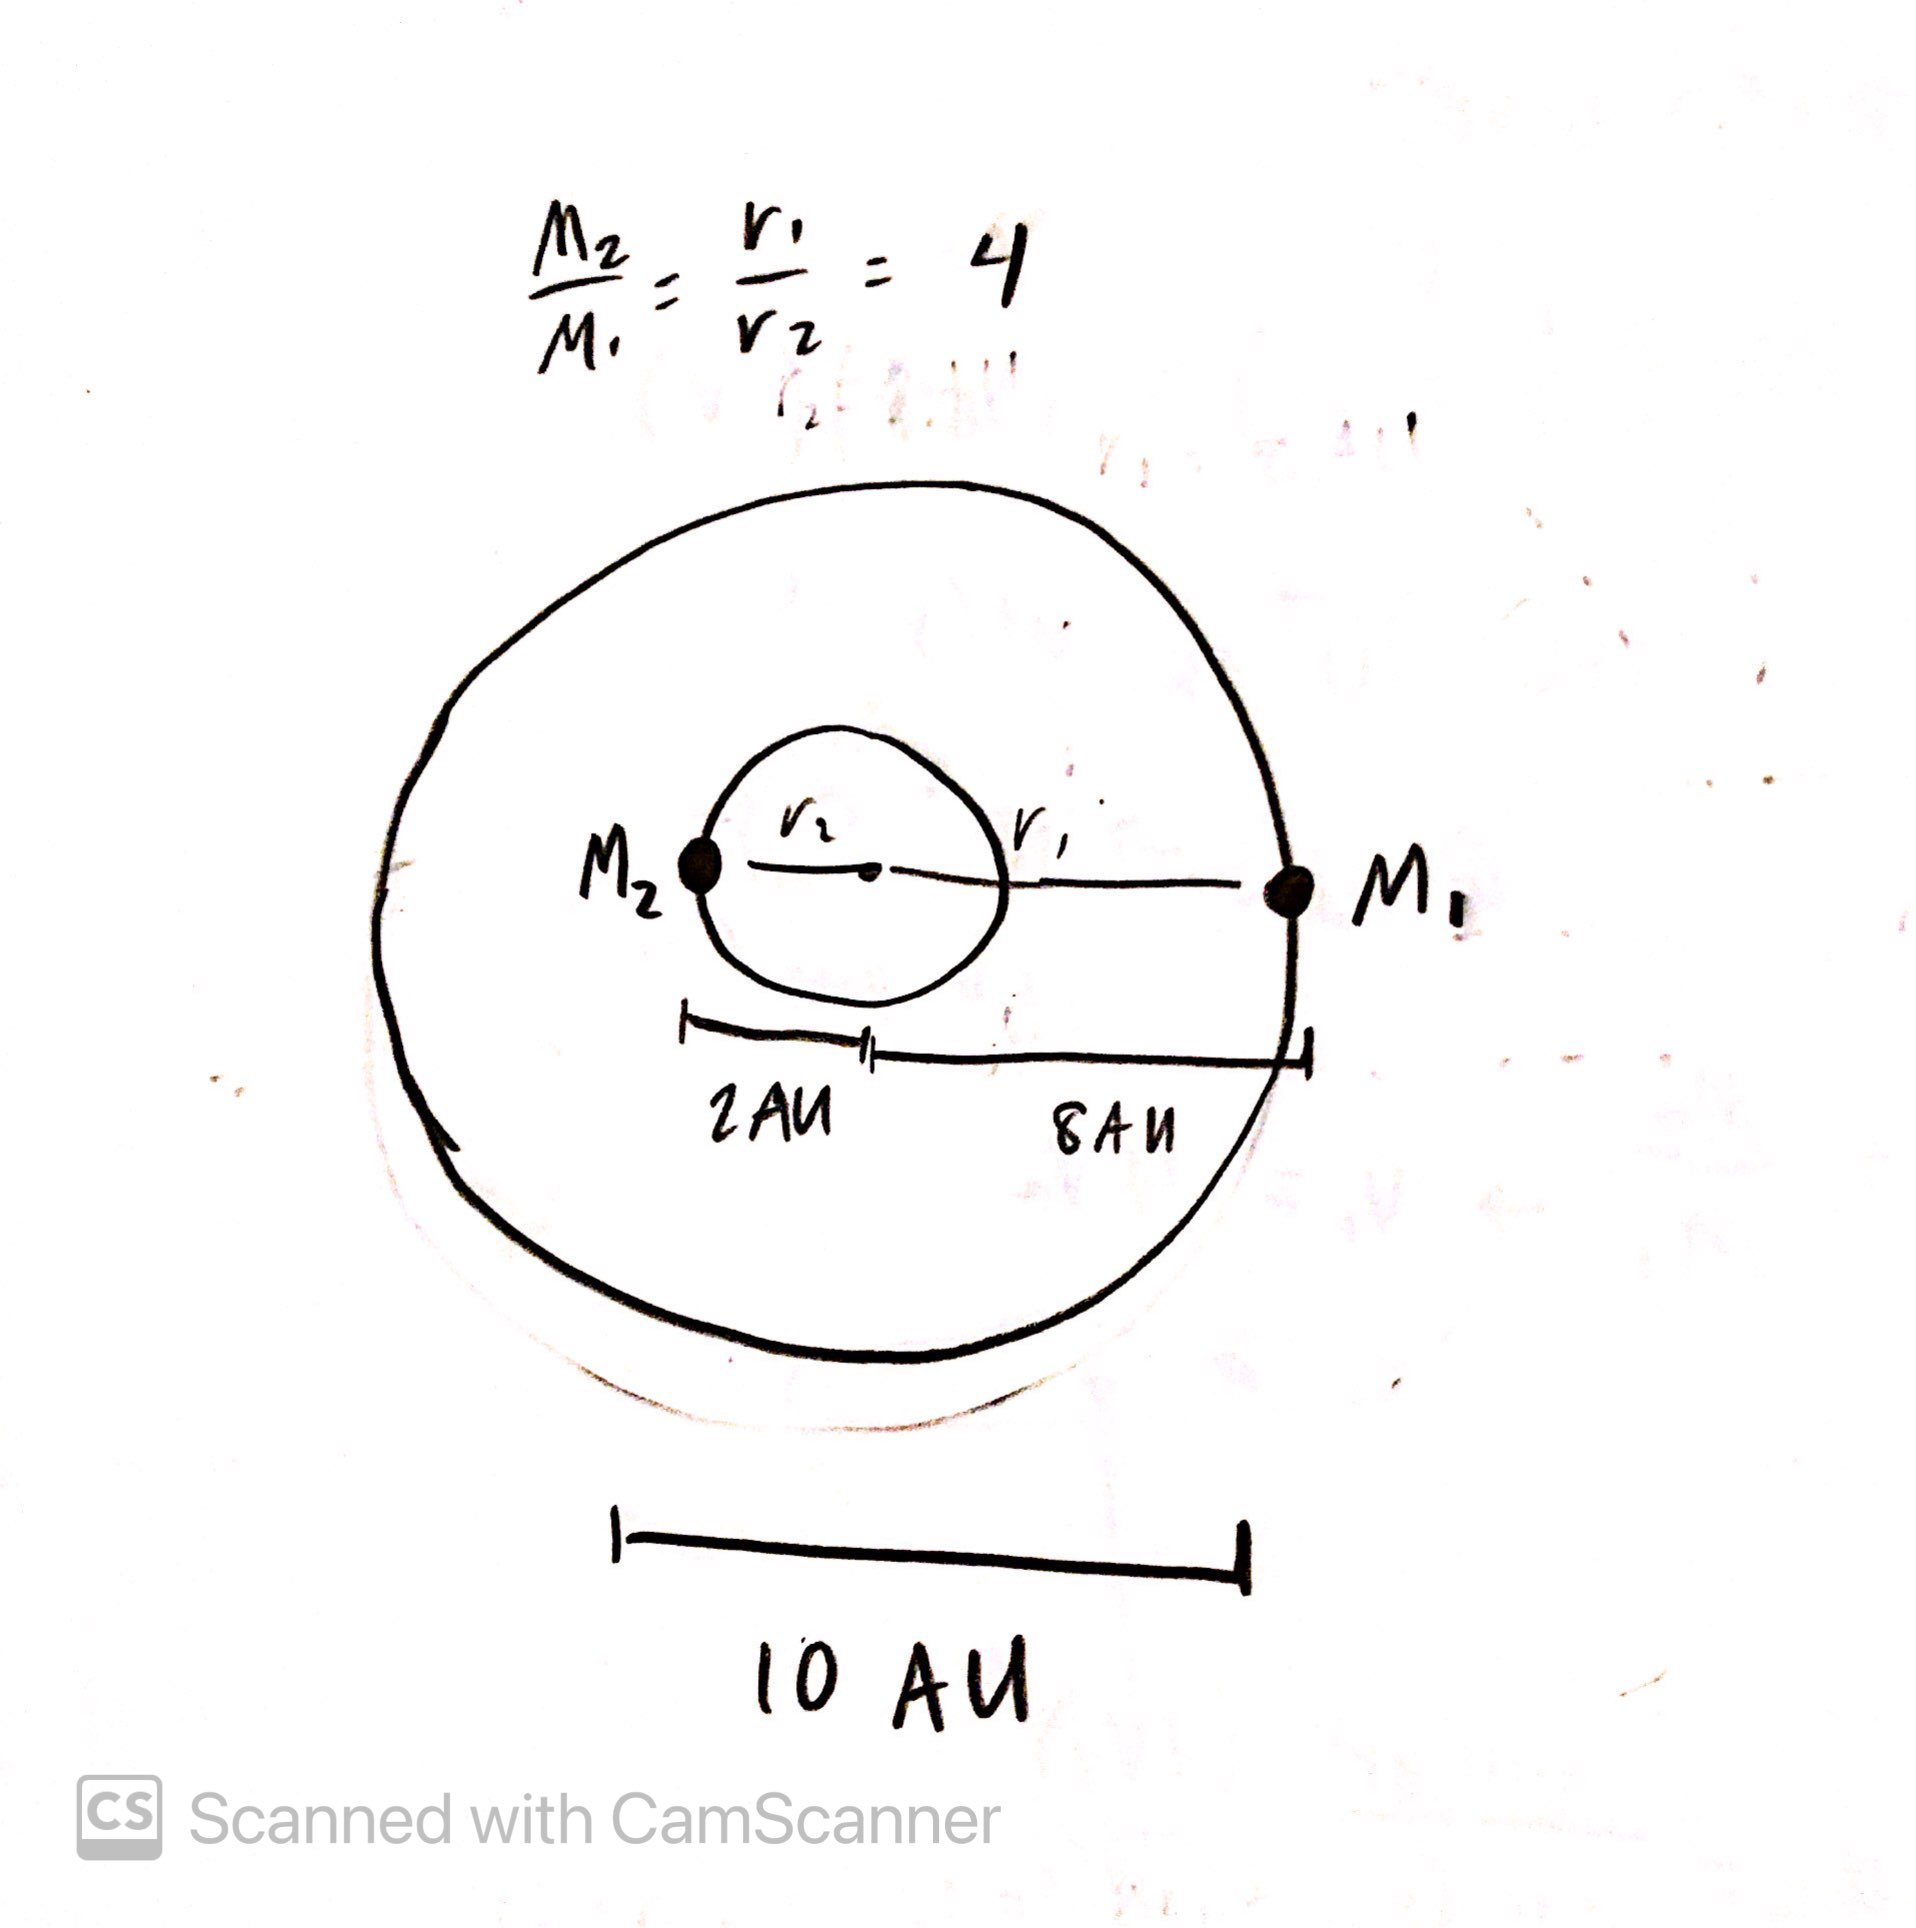
\includegraphics[width=0.4\textwidth]{problem3a.jpg}
    \end{figure}
    
    \questionpart Find period then plug into spectral binary equation.
        \begin{align*}
            M_1 + M_2	&=  \frac{A^3}{P^2}	\\
            5	&=  \frac{10^3}{P^2} \text{yr}	\\
            P   &=  \SI{14.14}{yr}   \\
            v_{1,max}   &=  \frac{2\pi*\SI{8}{AU}}{\SI{14.14}{yr}}  \\
            v_{1,max}   &=  \SI{3.37e6}{\metre\per\second}  \\
            v_{max} &=  \SI{3.37e6}{\metre\per\second}  + \SI{2e4}{\metre\per\second}   \\
            v_{max} &=  \SI{3.39e6}{\metre\per\second}  \\
            z   &=  \frac{v}{c} \\
            \frac{\SI{3.39e6}{\metre\per\second}}{\SI{3e8}{\metre\per\second}}    &=  \Delta / \SI{6563}{\angstrom} \\
            \Delta  &=	\SI{74}{\angstrom}	\\
            \lambda_{max}   &=  \SI{6563}{\angstrom} + \Delta  \\
            \lambda_{max}   &=  \boxed{\SI{6637}{\angstrom}}
        \end{align*}
    \questionpart Velocity curves.
    \begin{figure}[h]
        \centering
        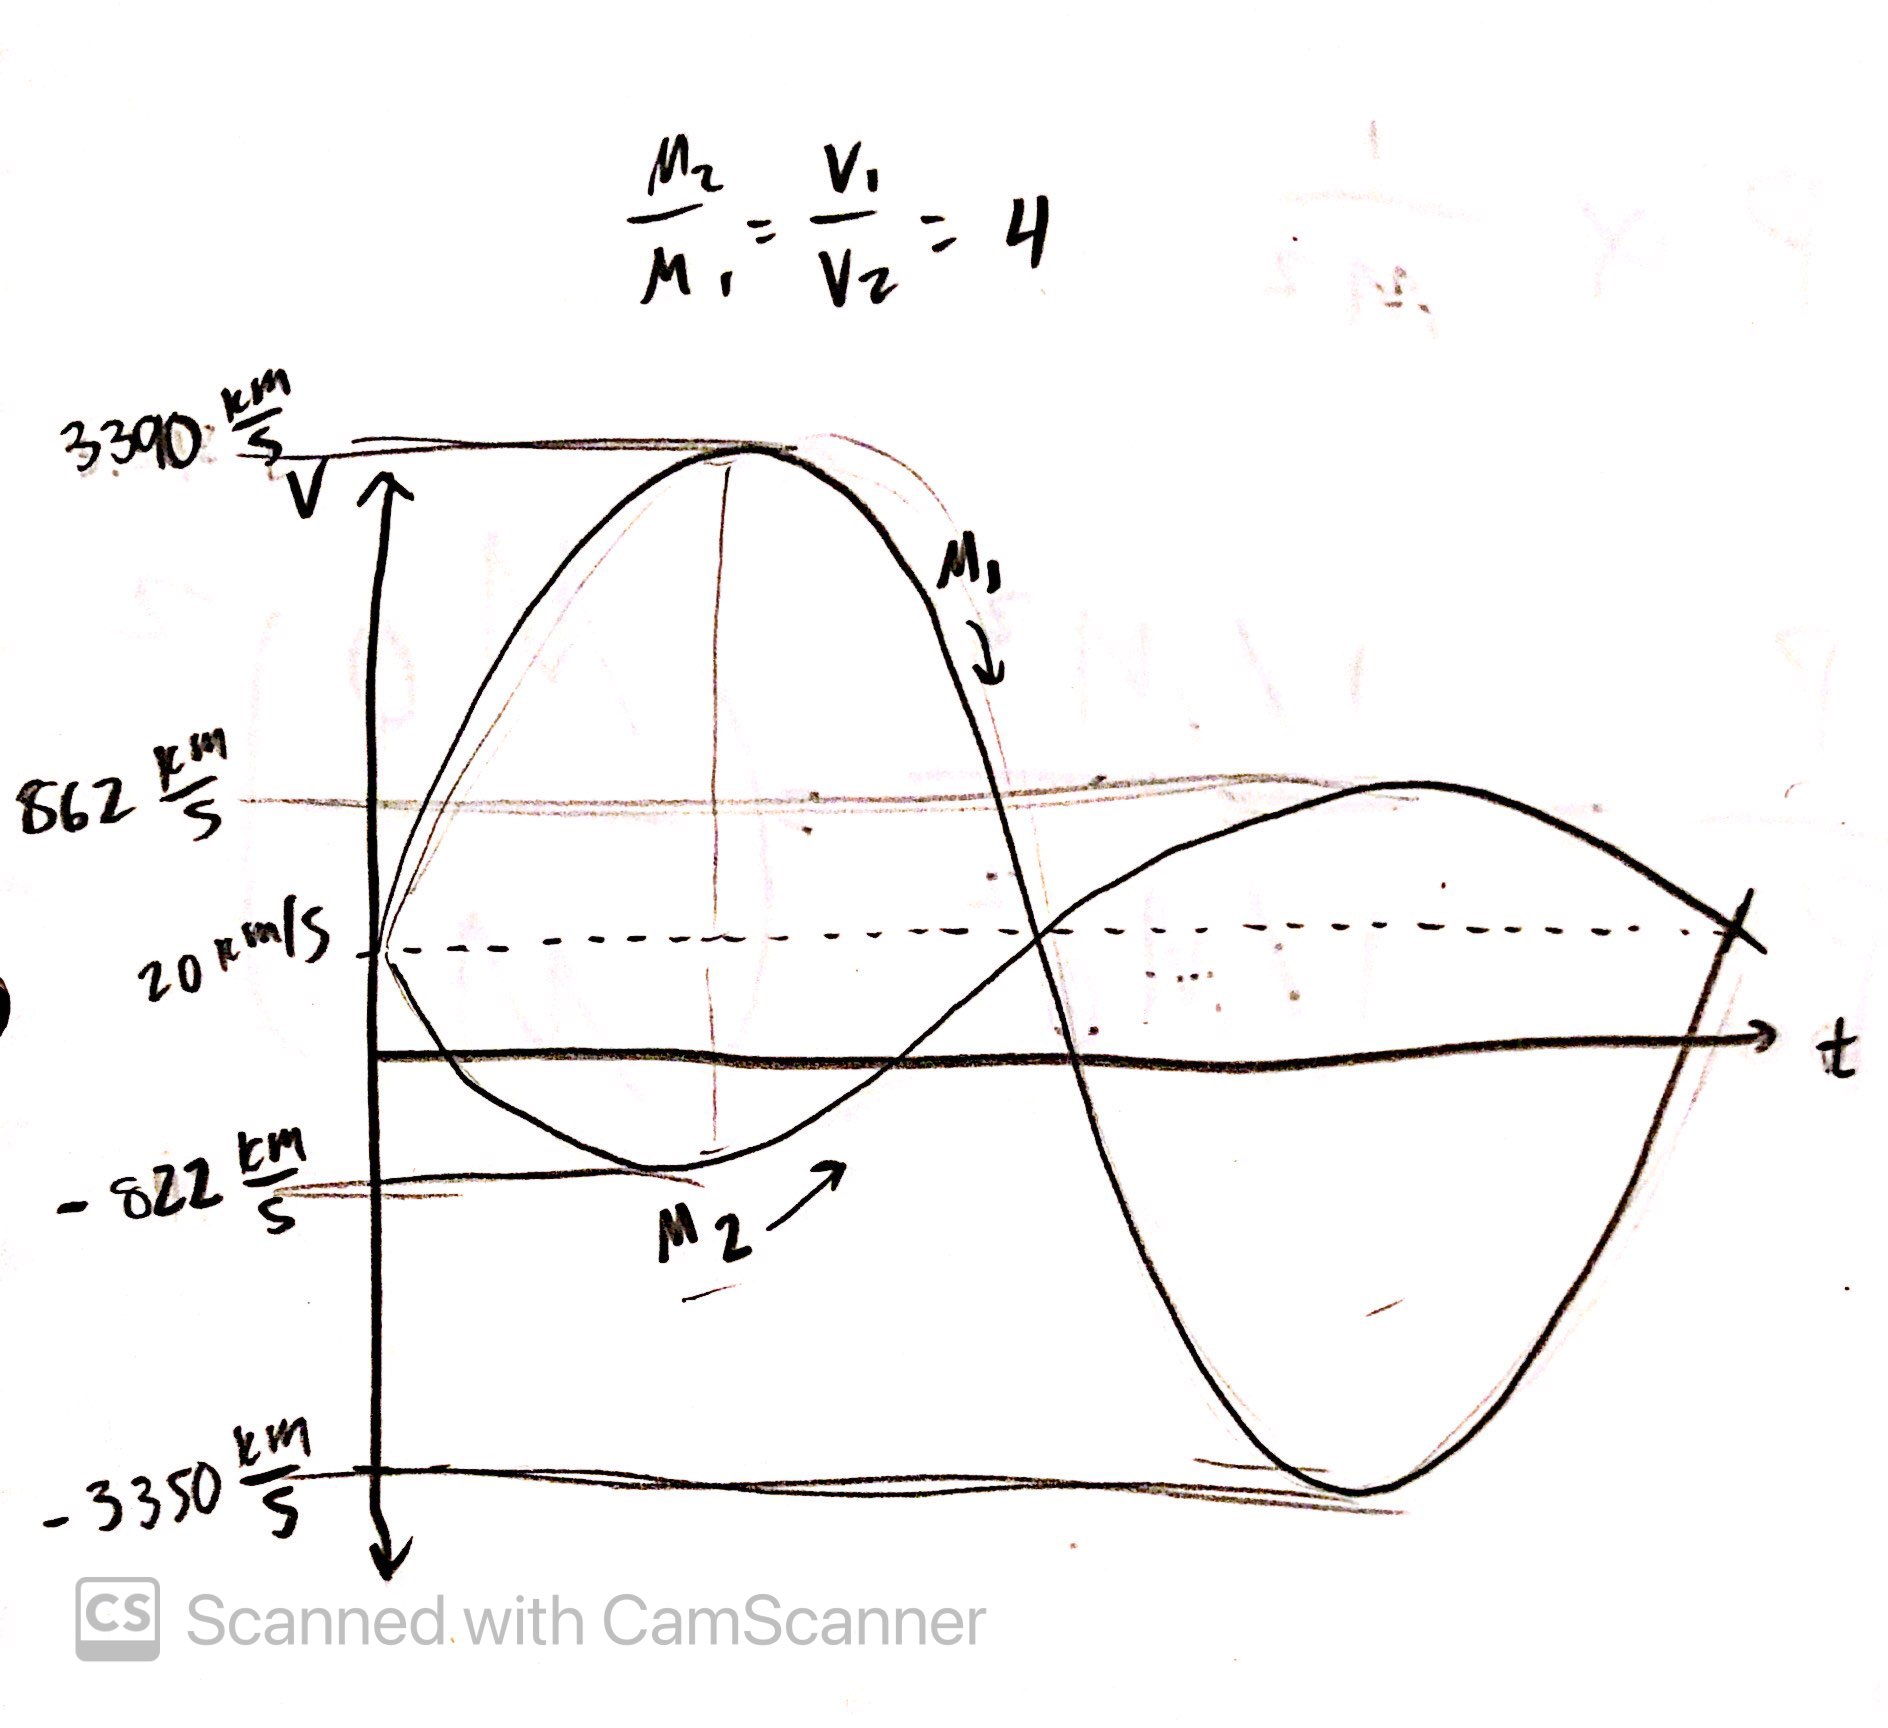
\includegraphics[width=0.4\textwidth]{problem3c.jpg}
    \end{figure}
    
    \questionpart If the inclination were actually 45 degrees, the plot would look a bit more flattened out as the velocity along the line-of-sight will be reduced when part of its movement is in the plane of the sky. However, the 
\end{alphaparts}

\question
Its inclination must be 90 degrees, that is, the orbital plane is in the line-of-sight. We know this because if it's an eclipsing binary, the stars block each other in our line of sight at some point, so they must be orbiting in that way.


\question
\begin{alphaparts}
    \questionpart Ratio of luminosities:
    \begin{align*}
        \frac{L_X}{L_Y}	&=	\frac{T_X^4 R_X^2}{T_Y^4 R_Y^2}	\\
        \frac{L_X}{L_Y}	&=	1 / (3^4 \vdot 4^2)	\\
        \frac{L_X}{L_Y}	&=	\boxed{1/1296}
    \end{align*}
    \questionpart The smaller star gets eclipsed at primary minimum so \fbox{Star X}.
    \questionpart It is a \fbox{total eclipse} because by definition the primary minimum is when the smaller star gets eclipsed so it will get entirely eclipsed.
    \questionpart  Ratio of depths:
    \begin{align*}
        \frac{\Delta F_{primary}}{\Delta F_{secondary}}	&=	\frac{T_X^4}{T_Y^4}	\\
        \frac{\Delta F_{primary}}{\Delta F_{secondary}}	&=	\boxed{1/81}
    \end{align*}
    \questionpart The depths of each eclipse stay the same since they are only proportional to the fourth power ratio of temperatures. Since in this case the more luminous star is smaller and gets fully eclipsed by the larger star, the graph of the eclipse fluxes shift downwards and the definition of primary and secondary eclipses switch.
\end{alphaparts}

\question
\begin{alphaparts}
    \questionpart $M_A / M_B = V_B / V_A = \boxed{4}$
    \questionpart $M_A + M_B = \frac{\SI{6}{yr} \vdot \SI{25000}{\metre\per\second}^3}{2\pi G} = \boxed{\SI{7.05e30}{\kilogram}}$
    \questionpart $5 M_B = \SI{7.05e30}{\kilogram}$ so $M_B = \boxed{\SI{1.41e30}{\kilogram}}$ and $M_A = \boxed{\SI{5.64e30}{\kilogram}}$.
    \questionpart Radii.
    \begin{align*}
        r_A	&=	\frac{1}{2} \SI{25}{\kilo\metre\per\second} \SI{24}{\hour}	\\
        r_A &=  \boxed{\SI{1.08e9}{\metre}}    \\
        r_B	&=	\frac{1}{2} \SI{25}{\kilo\metre\per\second} \SI{12}{\hour}	\\
        r_B	&=	\boxed{\SI{5.4e8}{\metre}}
    \end{align*}
    \questionpart $(T_s/T_l)^4 = (10^{5/-2.5} - 10^{9/-2.5}) / (10^{5/-2.5} - 10^{5.5/-2.5}) = 2.64$ so $T_B/T_A = \boxed{1.27}$.
\end{alphaparts}


\question
\begin{alphaparts}
    \questionpart \boxed{Yes.} You could estimate it by simply taking a constant density and then calculating pressure differences between shells of masses of width dr until you get to the center.
    \questionpart \boxed{No.} You need some measure of energy output like luminosity to estimate temperature of a blackbody.
\end{alphaparts}


\question
\begin{alphaparts}
    \questionpart Note $P_c \propto 1/M^2$ so $P = 1/M^2 P_\odot$.
    \begin{align*}
        P_{0.5}	&=	4 P_\odot	\\
        P_{10}	&=	0.01 P_\odot	\\
        P_{50}	&=	0.0004 P_\odot	\\
    \end{align*}
    \questionpart Note for thermal pressure we get $P = nKT$ so $T = P / nK$ so plug in previously found central pressures.
    \begin{align*}
        T_{0.5}	&=	4 P_\odot / nK	\\
        T_{10}	&=	0.01 P_\odot / nK	\\
        T_{50}	&=	0.0004 P_\odot / nK	\\
    \end{align*} 
\end{alphaparts}

\end{document}
